\documentclass[a4paper,12pt,bold,leqno,fleqn,a4]{scrartcl}

\renewcommand{\baselinestretch}{1.5}\normalsize

\usepackage{apacite}
\usepackage[round,longnamesfirst]{natbib}
\usepackage{bm}																									%matrix symbol
\usepackage{setspace}																						%Fu�noten (allgm.
\usepackage{hyperref}
%Zeilenabst�nde)
\usepackage{threeparttable}
\usepackage{lscape}																							%Querformat
\usepackage{graphicx}
\graphicspath{{material/}}

\usepackage{amsmath}
\usepackage{amssymb}
\usepackage{fancybox}																						%Boxen und Rahmen
\usepackage{appendix}
\usepackage{enumerate}
																					%EURO Symbol
\usepackage{tabularx}
\usepackage{longtable}																					%Mehrseitige Tabellen
\usepackage{color,colortbl}																			%Farbige Tabellen
\usepackage[left=2.5cm, right=2.5cm, top=2cm, bottom=3cm]{geometry} %Seitenr�nder
%\usepackage[normal]{caption2}[2002/08/03]												%Titel ohne float - Umgebung

\setlength{\skip\footins}{1.0cm}
\deffootnote[1em]{1.1em}{0em}{\textsuperscript{\thefootnotemark}}
\renewcommand{\arraystretch}{1.05}



\newenvironment{boenumerate}
{\begin{enumerate}\renewcommand\labelenumi{\textbf{(\theenumi)}}}
{\end{enumerate}}
\parindent0pt


\usepackage{graphicx}
\newcommand\sbullet[1][.5]{\mathbin{\vcenter{\hbox{\scalebox{#1}{$\bullet$}}}}}
\usepackage[export]{adjustbox}

\title{Causal Graphs}
\subtitle{-- Handout with definitions--}
\date{}

\begin{document}\maketitle\vspace{-2cm}

\section*{Basic definitions}

\begin{itemize}

\item A \textbf{node} represents a random variable labeled by letter. Observed random variables are marked by solid circle $\bullet$ and unobserved - by hollow circle \( \circ \).

\item An \textbf{edge} shows dependence between joining variables.

\item \textbf{Adjacent variables} are connected by an edge.

\item \textbf{Adjacent edges} meet at a variable.

\item \textbf{Directed edges} represent the causes by single-headed arrows.

\item \textbf{Parent/child} is the starting(tail)/ending(head) variable. Therefore, a directed edge represents a direct effect of a parent on a child.

\item \textbf{Root} is a variable that has no parent, or, in other words, exogenous variable determined only by forces outside of the graph.

\item \textbf{Sink} is a variable with no children.

\item \textbf{Path} is a sequence of adjacent edges.

\item \textbf{Directed path} is a path traced out entirely along arrows tail-to-head. If there is a directed path from A to B,  A is an \textbf{ancestor} of B; B is a  \textbf{descendant} of A.\\

\item \textbf{Directed acyclic graph (DAG)} is a graph with only arrows for edges and no feedback loops (i.e. no variable is its own ancestor or its own descendant):\\

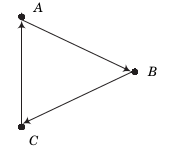
\includegraphics[trim=0 0 0 -1cm, center]{../material/fig-graph-with-cycle.png}

\item \textbf{Mutual dependence} of two variables on one or more common causes is shown by a curved and dashed bidirected edge:\\
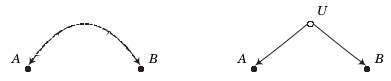
\includegraphics[trim=0 -1cm 0 -1cm, center]{../material/fig-graph-shorthand-unobserved-common-cause.png}

\end{itemize}

\section*{Basic patterns and strategies}

\textbf{Chain of mediation} is a relationship when A affects B through A's causal effect on C and C's causal effect on B.\\
\textbf{Mutual dependence} is a relationship when A and B are both caused by  (graph b).\\
\textbf{Mutual causation} is a relationship when A and B both causes of C. \\
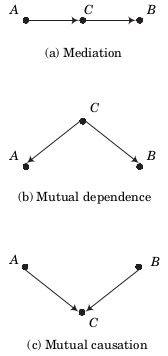
\includegraphics[trim=0 -1cm 0 -1cm, center]{../material/fig-graph-basic-causal-relationships.png}
\textbf{Confounding variable} is a variable that affects both the dependent and independent variable (in our example, variable C on the graph b).\\
\textbf{Collider} is a variable that has two arrows running into it (in our example, variable C on the graph c).\\
\textbf{Conditioning} as a modeling strategy means transforming one graph into a simpler set of component graphs where fewer causes are represented.\\
\textbf{Back-door path} is a path between any causally ordered sequence  of two variables that include a directed edge that points to the first variable. \\
\textbf{Back-door criterion} is a set of conditions used to determine whether or not conditioning on a given set of observed variable will identify the causal effect. The causal effect is identified by conditioning on a set of variables Z if and only if all back-door paths between the causal variable and the outcome variable are blocked after conditioning on Z. All back-door paths are blocked by Z if and only if each back-door path:
\begin{enumerate}
\item contains a chain of mediation A $\rightarrow$ C $\rightarrow$  B where the middle variable C is in Z, or
\item contains a fork of mutual dependence A $\leftarrow$ C $\rightarrow$ B, where the middle variable C is in Z, or
\item contains an inverted fork of mutual causation A $\rightarrow$ C $\leftarrow$  B, where the middle variable C and all of C's decendents are not in Z.
\end{enumerate}

\nocite{Morgan.2014}
\nocite{Pearl.2009}

\bibliographystyle{apacite}
\bibliography{../../../submodules/bibliography/literature}

\end{document}
